\documentclass[tikz,border=2pt]{standalone}
\usepackage{amsmath,amssymb}
\usepackage{pgfplots}
\pgfplotsset{compat=1.18}

\begin{document}
% Two MGFs: Bern(1/2), finite for every t, and Exp(1), finite only for t < 1. Both pass through
% (0, 1) because M(0) = E[1] = 1.
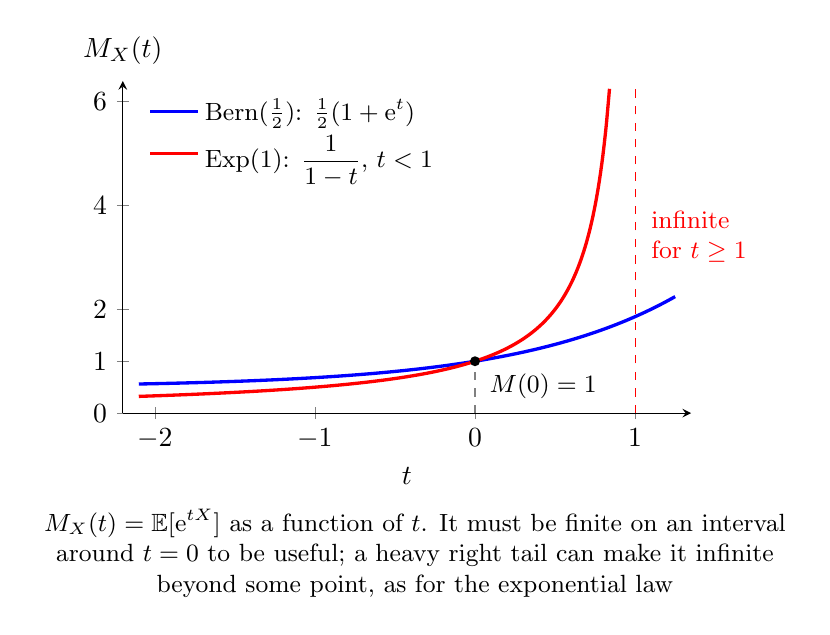
\begin{tikzpicture}
	\begin{axis}[
		axis lines=left, xmin=-2.2, xmax=1.35, ymin=0, ymax=6.4,
		xtick={-2,-1,0,1}, ytick={0,1,2,4,6},
		xlabel={$t$}, ylabel={$M_X(t)$}, ylabel style={rotate=-90, anchor=south, at={(axis description cs:0,1.02)}},
		samples=140, smooth, width=8.8cm, height=5.8cm, clip=false,
		legend style={draw=none, fill=none, font=\small, at={(0.03,0.98)}, anchor=north west}, legend cell align=left
		]
		\addplot[blue, very thick, domain=-2.1:1.25] {(1+exp(x))/2};
		\addlegendentry{$\operatorname{Bern}(\tfrac12)$: $\tfrac12(1+\mathrm{e}^t)$}
		\addplot[red, very thick, domain=-2.1:0.84] {1/(1-x)};
		\addlegendentry{$\operatorname{Exp}(1)$: $\dfrac1{1-t}$, $t<1$}
		\draw[red, dashed] (axis cs:1,0) -- (axis cs:1,6.3);
		\draw[gray, dashed] (axis cs:0,0) -- (axis cs:0,1);
		\fill[black] (axis cs:0,1) circle (1.8pt);
		\node[anchor=north west, font=\small] at (axis cs:0.03,0.95) {$M(0)=1$};
		\node[red, anchor=west, font=\small, align=left] at (axis cs:1.04,3.4) {infinite\\ for $t\ge1$};
	\end{axis}
	\node[anchor=north, font=\small, align=flush center, text width=9.6cm] at ([yshift=-2pt]current axis.outer south) {$M_X(t)=\mathbb{E}[\mathrm{e}^{tX}]$ as a function of $t$. It must be finite on an interval around $t=0$ to be useful; a heavy right tail can make it infinite beyond some point, as for the exponential law};
\end{tikzpicture}
\end{document}
